% Template for ICASSP-2010 paper; to be used with:
%          mlspconf.sty  - ICASSP/ICIP LaTeX style file adapted for MLSP, and
%          IEEEbib.bst - IEEE bibliography style file.
% --------------------------------------------------------------------------
\documentclass{article}
\usepackage[utf8]{inputenc}
\usepackage[english]{babel}
\usepackage{amsmath,graphicx,02460}
\usepackage[acronym,nomain,nonumberlist,nopostdot,nogroupskip]{glossaries}
%% HOW TO CREATE AN ACRONYM
% \newacronym{1}{2}{3}
% 1: the LaTeX name of the acronym, you use this when you mention the acronym in the text with \gls{}, \Gls{} or \glspl{}
% 2: the acronym that is displayed
% 3: the full text what the acronym stands for, that is printed when \gls{} is used for the first time for this acronym
% example: \newacronym{ppd}{PPD}{Pharmaceutical Process Development}
% Usage in code then is: \gls{ppd} 
% \glspl{ppd} would give you an s after the acronym+text. pl = plural
% \Gls{} forces the first letter to be uppercase

% TO PRINT ACRONYM LIST
% use this command in main.tex:
% \printglossary[type=\acronymtype ,title=List of abbreviations]
% and make sure command \makeglossaries has been called before

\newacronym{ffnn}{FFNN}{feed-forward neural network}
\newacronym{vae}{VAE}{variational auto-encoder}
\newacronym{scvae}{scVAE}{single-cell variational auto-encoder}
\newacronym{scrna-seq}{scRNA-seq}{single-cell RNA sequencing}
\newacronym{rna-seq}{RNA-seq}{RNA sequencing}
\newacronym{lr}{LR}{latent representation}
\newacronym{pca}{PCA}{principal component analysis}
\newacronym{tsne}{tSNE}{t-distributed stochastic neighbor embedding}
\newacronym{elbo}{ELBO}{evidence lower bound}
\newacronym{ngs}{NGS}{next-generation sequencing}
\newacronym{pbmc}{PBMC}{peripheral blood mononuclear cells}
\newacronym{gmvae}{GMVAE}{gaussian mixture variational auto-encoder}
\usepackage{fancyhdr}
\renewcommand{\headrulewidth}{0pt}
\usepackage{hyperref}

\toappear{02456 Deep Learning, DTU Compute, Fall 2020}

% page number
\pagestyle{fancy}
\fancyhf{}
\rfoot{\small\thepage}

% Example definitions.
% --------------------
\def\x{{\mathbf x}}
\def\L{{\cal L}}

% Title.
% ------
\title{\Large{Exploring variational autoencoders potential to classify single-cell RNA-seq data}}
%
% Single address.
% ---------------

\name{Bego\~na Bolos$^{1}$, Felix Pacheco $^1$, Paula Rodriguez$^1$, Laura Sans-Comerma$^1$, Ole Winther$^{2,3}$}
\address{\small{$^1$ DTU Bioinformatics, Technical University of Denmark,$^2$ The Bioinformatics Centre, Department of Biology, University of Copenhagen, \\
\small{$^3$ DTU Compute, Technical University of Denmark}}}
%
% hyperref
\hypersetup{
    colorlinks=true,
    linkcolor=black,
    filecolor=black,      
    urlcolor=cyan,
    citecolor=black,
    
}

\begin{document}

\maketitle
% -------------abstract-------------------
\begin{abstract}
Deep generative models, such as \glspl{vae} can be used to analyze \gls{scrna-seq} data, generating \glspl{lr} which capture most variability of gene expression levels.
The library \gls{scvae} applies \glspl{vae} on raw \gls{scrna-seq} data, omitting all pre-processing steps and producing a latent representation useful for downstream analyses \cite{gronbech2020}.
In this study, the potential of deep generative models such as \gls{scvae} has been evaluated on a cell type classification problem, using 10x-PBMC-68k data set \cite{zheng2017a}. 
For this purpose, a \gls{lr} of the \gls{scrna-seq} data has been generated with \gls{scvae} and subsequently inputted into a \gls{ffnn} model to classify the cell types.
This model has been compared to other two \glspl{ffnn}
trained with (1) sparse raw data and (2) the components resulting from applying \gls{pca} on the sparse raw data.
Contrary to our hypothesis, results do not show clear differences in classification accuracy among the three different training inputs.
These findings should be further validated with larger sample sizes to truly assess the potential of \glspl{vae} to classify \gls{scrna-seq} data.
%This outcome might be affected by the small sample size used, which could not be increased due to limited computational resources.
\end{abstract}
%
\begin{keywords}
Deep generative models, variational auto-encoders, feed-forward networks, single-cell RNA-seq, cell type classification.
\end{keywords}
%
% ---------------intro-----------------
\section{Introduction}
\label{sec:intro}
The development of \gls{ngs} technologies in the recent years has provided highly valuable insights into biological systems from cancer genomics to diverse microbial communities.
Data resulting from \gls{rna-seq}, typically performed for the study of the transcriptome or analysis of gene expression levels, represents an average of gene expression patterns across thousands to millions of cells, which can hide potentially significant and biologically important differences between cells. 
\gls{scrna-seq} has taken transcriptome profiling to the next level, analyzing individual cells by uncovering their gene expression variability, providing a higher resolution of cellular differences \cite{Olsen2018}. \\ 
%This technique allows addressing topics like cell type identification, understanding tissue heterogeneity, detection of cellular and molecular changes in diseased tissue or tracing cell lineage and differentiation
%\cite{Olsen2018}.\\ 

%cell type identification
%In particular, cell type identification from scRNA-seq data has become relevant for understanding how tissues function and underlying mechanisms in pathological states. 
%Features used to define cell types include lineage, location, morphology, activity, interactions with other cell types, epigenetic state, responsiveness to certain signals, and molecular composition (including mRNA and protein levels) 
% However, few reliable markers exist for any given cell type, and hidden diversity remains even with well-established markers (e.g., cluster of differentiation (CD) markers in immune cells) (hwang 2018).
\noindent Transcriptome profiling can be used to classify cell types, partitioning the data into clusters of single cells, where each cluster is defined by a unique gene expression signature relative to other clusters \cite{Shekhar2019, Hwang2018}. 
However, the human body contains approximately 40 trillion cells and complex mammals contain $\sim$ 30,000 genes in their genomes. 
Hence, data from \gls{scrna-seq} experiments is often high dimensional, but also sparse, introducing challenges in computational analyses.\\

%-Dealing with dimensionality
%When comparing cells in a high dimensional gene expression space, distances between cells become more homogenous, making it difficult to distinguish differences between populations from variability within a population.

\noindent Dimensionality reduction is one of the approaches used to deal with the high-dimensional gene expression data obtained from \gls{scrna-seq} experiments, in which the data is projected into a lower dimensional space. 
\gls{pca} or \gls{tsne} are commonly used.
%For instance, t-SNE is implemented in the popular Cell Ranger pipeline (10× Genomics) and in Seurat R package (http://satijalab.org/seurat/).
Furthermore, machine learning algorithms have been used for identifying cell types as unsupervised clustering problem in different studies, including algorithms as K-means, hierarchical clustering, density-based clustering or graph-based clustering. 
Clustering algorithms are commonly combined with dimensionality reduction and/or feature selection to identify cell types \cite{andrews2018, Peyvandipour2020}. \\
 
%Methods SC328 and Seurat25 use a combination of feature selection, dimensionality reduction, and clustering algorithms to identify the cell types. 

%- scVAE library
\noindent Recently, new methods that model the gene expression levels directly as counts have been developed, skipping the pre-processing for analyzing \gls{scrna-seq} data \cite{Lopez2018, Eraslan2019}. 
Particularly, \glspl{vae} are deep generative models which use many different data distributions from the training data using unsupervised learning. 
\glspl{vae} learn compressed \glspl{lr} of the data by de-noising the input using an encoder-decoder structure. 
Thus \glspl{vae} capture most of the variance from the data by generating \glspl{lr} with a lower dimensionality than the input.
The reconstruction error is minimized by computing the \gls{elbo} \cite{kingma2014a}.\\
%which stores useful information about the type of output the model needs to generate
% More  precisely,the training is done by maximizing the lower bound of thedata log-likelihood. VAEs learn compressed LRs of the databy de-noising the input using the encoder-decoder structure,which store useful information about the type of output themodel needs to generate

\noindent Some advantages of \gls{vae} approach are its probabilistic nature and the fact that different likelihood functions for modelling the data distributions can be applied. This method has been recently applied for modelling directly raw count data from \gls{rna-seq} \cite{Way2017} or \gls{scrna-seq} experiments for cell-type classification \cite{gronbech2020}. 
In the last case, the publicly available library \underline{\href{https://github.com/scvae/scvae}{\gls{scvae}}} offers the possibility of modelling \gls{scrna-seq} data to the user by choosing different the likelihood functions, and giving vast range of the hyperparameters values to tune \cite{gronbech2020}.\\

\noindent In this study, the potential of \gls{vae} generative models will be explored on a cell type classification problem based on available framework for unsupervised modelling \gls{scvae} \cite{gronbech2020}. 
To do so, a \gls{lr} of \gls{scrna-seq} data, generated with \gls{scvae}, will be used to train a \gls{ffnn} to classify the cell types.
These results will be compared with (1) a \gls{ffnn} classifier trained with sparse raw data and (2) a \gls{ffnn} classifier after applying dimensionality reduction through \gls{pca}.
% To do so, the latent representation of the data will be trained by a FFNN to classify the cell types in order to be able to compare these results with (1) \gls{ffnn} classification used on sparse raw data and (2) \gls{ffnn} classification after performing a dimensionality reduction through \gls{pca}.\\

% -------------methods-------------------
\section{Methods}
\label{sec:methods}


\noindent The main goal of this study is to validate the ability of \glspl{vae} to classify \gls{scrna-seq} data. 
To do so, a workflow was designed, as seen in figure \ref{figure:overview}.
For the study, three data sets must be obtained: (1) raw data, (2) \glspl{lr} of the raw data obtained by running \gls{scvae} and (3) resulting features from computing \gls{pca} on the raw data, obtaining the same number of components as \gls{lr} dimensions used in data set (2).
Subsequently, all three data sets will be fed to a simple \gls{ffnn} to classify the cell type. \\

\begin{figure}[htp]
    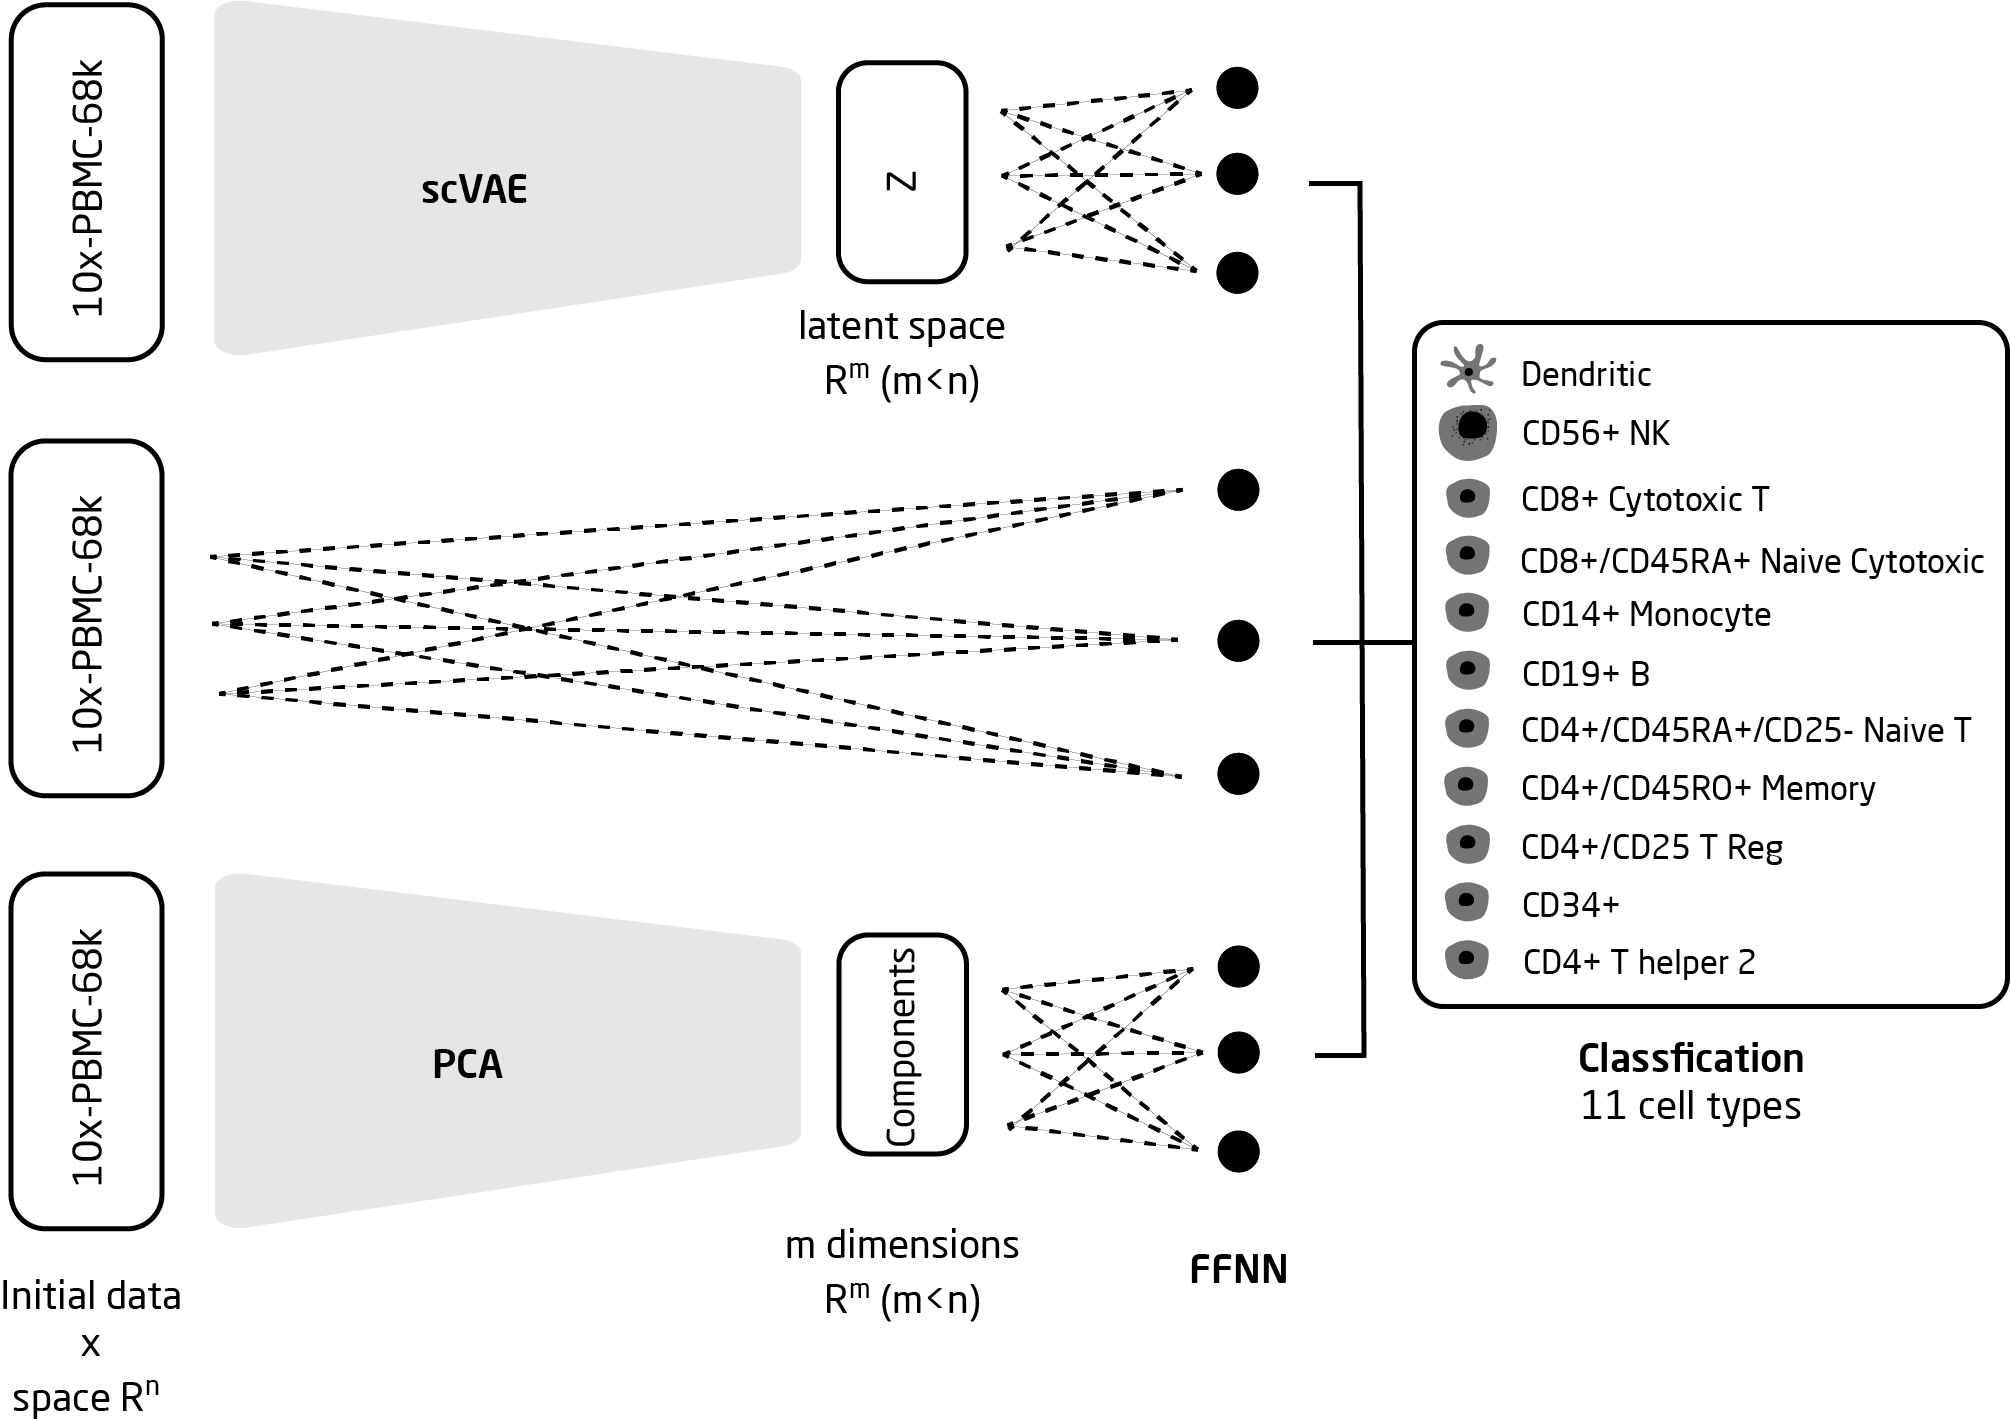
\includegraphics[width=0.475\textwidth]{02456_report/images/workflow_report.png}
    \caption{\small{Overview of the workflow}}
    \label{figure:overview}
\end{figure} 

% ------------dataset--------------------
\subsection{Data set}
\label{sec:dataset}

\noindent The data set used in this study is the \gls{pbmc} from 10X Genomics Fresh Donor A (10x-PBMC-68k), used in Zheng, et al. 2017 \cite{zheng2017a}. 
The data set consists of \gls{scrna-seq} data from $\sim 68,000$ cells, that checks counts for $\sim 32,000$ genes. 
It was sequenced using Illumina NextSeq 500 High throughput technologies with $\sim 20,000$ reads per cell, with a final number of reads of $\sim 1,400$M. 
The sequencing output was aligned using the \textit{hg19} transcriptome. 
In supplementary figure S1, two \gls{tsne} projections of the data set can be observed.\\ % In the projection colored by k-means clustering, it is shown that the data has a good clustering in 10 clusters.\\

\noindent Due to time and computational power restraints, it was decided that the study would be performed with a subset of the data set. 
The models and analyses were done with 2\% of the total number of cells, being 1,300 cells. 
However, after seeing the results, new models were performed, this time with a subset of 25\% of the total number of cells, being 15,000 cells. \\
Nonetheless, it is important to note that only the \glspl{lr} with the subset of 15,000 cells could be generated. 
The sparse, raw \gls{scrna-seq} subset of 15,000 cells could not be obtained despite considerable efforts and therefore \gls{pca} could not be performed on this subset either.


% -------------vae-------------------
\subsection{Variational Auto-Encoders}
\label{sec:vae}

\noindent As mentioned above, \gls{scvae} was run on a subset of the 10x-PMBC-68k data set containing 1,300 cells using different hyperparameters. %, 16 \glspl{lr} were obtained.
%\noindent To inspect the importance of the \gls{lr} dimension, different \gls{lr} were computed with four different latent dimensions. 
The different models were computed by combining two hyperparameters: the number of hidden units and the dimensions of the \glspl{lr}. 
Combining the number of hidden units, ($H\epsilon[100, 250, 500, 1000]$); and the dimensions of the \glspl{lr}, ($Z\epsilon[10, 25, 50, 100]$), 16 models were generated.
Subsequently, 4 more \gls{scvae} models, using the outperforming number of hidden units for each of the four latent dimensions, were run on a larger subset of 10x-PMBC-68k data containing 15,000 cells. \\

\noindent Other hyperparameters were left fixed for all models, as shown in table \ref{tab:scvae_fixed}. 
Since \gls{scrna-seq} data represents different cell types it is desirable to be able to classify it in different classes, or in this case, cell types. 
For this reason \gls{gmvae} was used as the model to fit the output. 
The likelihood function chosen to model the count data was the negative binomial function, following the results shown in Grønbech, et al. 2020 \cite{gronbech2020}.\\


% 2 table fixed parameters for scvae and ffnn

\begin{table}[htp]
\caption{\small{Fixed parameters for the all the trained models. (*) Split fraction refers to the fraction of the subset used for training. The remaining fraction is equally divided for validation and test. }}
\vspace{0.25cm}
\small
\centering
\begin{tabular}{ll}
    \hline
    Parameter & Fixed value \\
    \hline
    Model & GMVAE  \\
    Likelihood function & Negative binomial \\
    Epochs & 100 \\
    Split Fraction (*) & 0.8 \\
    Clusters & 11 \\
    Learning rate & $10^{-4}$ \\
    Hidden layers & 1 \\
    \hline
\end{tabular}
%\vspace{0.35cm}
\label{tab:scvae_fixed}
\end{table}


% --------------pca------------------
\subsection{Principal component analysis}
\label{sec:pca}
In order to compare the generated \glspl{lr} with simpler dimensionality reduction techniques, a subset of 10x-PMBC-68k data set containing 1,300 cells was used to perform \gls{pca}. 
For the reasons described in \textit{Methods} section \ref{sec:dataset}, \gls{pca} could only be performed on this subset, and not on the one with 15,000 cells.
Firstly, data standardization was performed with the \emph{StandardScaler} library, which standardizes features, or genes in this case, by removing the mean and scaling to unit variance. 
Secondly, \emph{\gls{pca}} library was used in order to perform the dimensionality reduction of the subset \cite{scikit-learn}.
In order to obtain a comparable output with \gls{scvae} latent representations, the number of components $k$, was set to $k\epsilon[10, 25, 50, 100]$. 
%After checking the variance explained in each of the four \gls{pca}, the result was stored in a data frame to carry out the \gls{ffnn}.
After applying \gls{pca}, the resulting components were stored to be used as input for the \gls{ffnn} classifier.

% --------------ffnn------------------
\subsection{Feed-forward neural network}
\label{sec:ffnn}
Cell type classification was carried by a \gls{ffnn} model, trained on the three data sets previously described.
For each latent dimension, only the \gls{lr} generated by the outperforming \gls{scvae} model was used, hence four \gls{scvae} input sets were used to train the network. 
Likewise, four \gls{pca} input sets were used to train the network, containing the same number of components as dimensions used in the \glspl{lr}.
%trained on (1) raw \gls{scrna-seq} data, (2) \gls{pca} components and (3) \glspl{lr} generated by \gls{scvae}.
%Cell type classification from \gls{pca} dimensionality reduction is compared with \gls{scvae} and raw data after performing \gls{ffnn}.  
\gls{ffnn} architecture was constructed with PyTorch \cite{pytorch}, using fixed parameter values shown in table \ref{tab:ffnn_fixed} for all three input sets used.
It was decided to maintain a simplistic \gls{ffnn} architecture for all input sets, while letting most of the complexity to be included in \gls{scvae} model.
Some parameters, such as Xavier Glorot initialization and Adam optimizer were selected based on literature \cite{gronbech2020, Eraslan2019, Ma2019, Johansen2019}. 
%assuming that \gls{pca} and \gls{scvae} contain most part of the variability of the data.
The data set was randomly split in 80\% training, 10\% validation and 10\% test. 
Model training was performed with the fixed values contained in table \ref{tab:ffnn_fixed}. 

\begin{table}[htp]
\caption{\small{Fixed parameters for \gls{ffnn} architecture and training. (*) ReLU function was used as activation function for the hidden layer, while Softmax function was used for the output layer. (**) The remaining fraction of the data set was equally divided for validation and test.}}
\vspace{0.25cm}
\small
\centering
\begin{tabular}{ll}
\hline
Architecture Parameters    & Value        \\
\hline
Initialization    & Xavier Glorot                 \\
Hidden layers & 1             \\
Hidden units     & 516                \\
Output classes     & 11               \\
Activation function     & ReLU/Softmax (*)                \\
& \\
\hline
Training Parameters    & Value        \\
\hline
Batch size    & 10                 \\
Epochs     & 100                \\
Training fraction (**)    & 0.8                \\
Optimizer     & Adam               \\
Learning rate & $10^{-4}$             \\
Loss criterion     & Cross Entropy Loss \\
\hline
\end{tabular}
\label{tab:ffnn_fixed}
\end{table}


% ------------results--------------------
\section{Results}
\label{sec:results}

\noindent To study the benefits of using \glspl{lr} to classify cell types with \gls{scrna-seq} data, a classification task was carried by a \gls{ffnn} trained on the \glspl{lr} generated with \gls{scvae}.
The \gls{ffnn} classifier was also trained with two other data inputs: (1) raw data and (2) the $k$ principal components resulting from applying \gls{pca}.
These different inputs were included in the present study to assess whether the use of \glspl{lr} for classification outperforms the use of raw data or classical dimensionality reduction techniques such as \gls{pca}.

% ------------ scvae --------------------
\subsection{Generation of latent representations of the data}
\label{sec:results_scvae}

\noindent The \glspl{lr} were evaluated based on the \gls{elbo} and Clustering Rand Index.
These two parameters were used since they provide information on the training quality and how suitable is the \gls{lr} for clustering cell types, respectively. 
The results of the different models can be seen in table \ref{tab:16_models}.
As it can be observed, the obtained Rand Index and \gls{elbo} values are considerably low.
\begin{table}[h]
\caption{\small{Initial \gls{scvae} 16 models test performance comparison from 1,300 cells subset. Z = latent dimensions; H = hidden units.}}
\vspace{0.4cm}
\small
\centering
\label{tab:16_models}
\begin{tabular}{rrrrr}
\hline
Model & Z & H & ELBO    & Rand Index \\ \hline
   &                                     &          & &    \\ 
1     & 10                                          & 100          & -5971.4 & 0.033      \\ 
2     &                                           & 250          & -4420.9 & 0.118      \\ 
3     &                                           & 500          & -3139.4 & 0.058      \\ 
4     &                                          & 1000         & -2860.9 & 0.045      \\ 
   &                                     &          & &    \\ 
5     & 25                                          & 100          & -5030.0 & 0.037      \\ 
6     &                                         & 250          & -3152.0 & 0.011      \\ 
7     &                                         & 500          & -2704.2 & 0.110      \\ 
8     &                                         & 1000         & -2605.3 & 0.090      \\ 
   &                                     &          & &    \\ 
9     & 50                                          & 100          & -4519.8 & 0.098      \\ 
10    &                                        & 250          & -2868.5 & 0.111      \\ 
11    &                                           & 500          & -2567.1 & 0.073      \\ 
12    &                                           & 1000         & -2513.3 & 0.092      \\ 
   &                                     &          & &    \\ 
13    & 100                                         & 100          & -4144.3 & 0.004      \\ 
14    &                                          & 250          & -2597.5 & 0.010      \\ 
15    &                                          & 500          & -2387.5 & 0.106      \\ 
16    &                                         & 1000         & -2437.8 & 0.014      \\
   &                                     &          & &    \\ \hline
\end{tabular}
\vspace{0.25cm}
\end{table}

\noindent Given that the models obtained to generate \glspl{lr} showed low values of Rand Index and \gls{elbo}, the outperforming four \gls{scvae} models were re-computed with a larger subset of 10x-PBMC-68k data set, containing 15,000 cells. 
The results can be observed in table \ref{tab:17-20_models}.\\

\begin{figure*}[t!]
\centering
    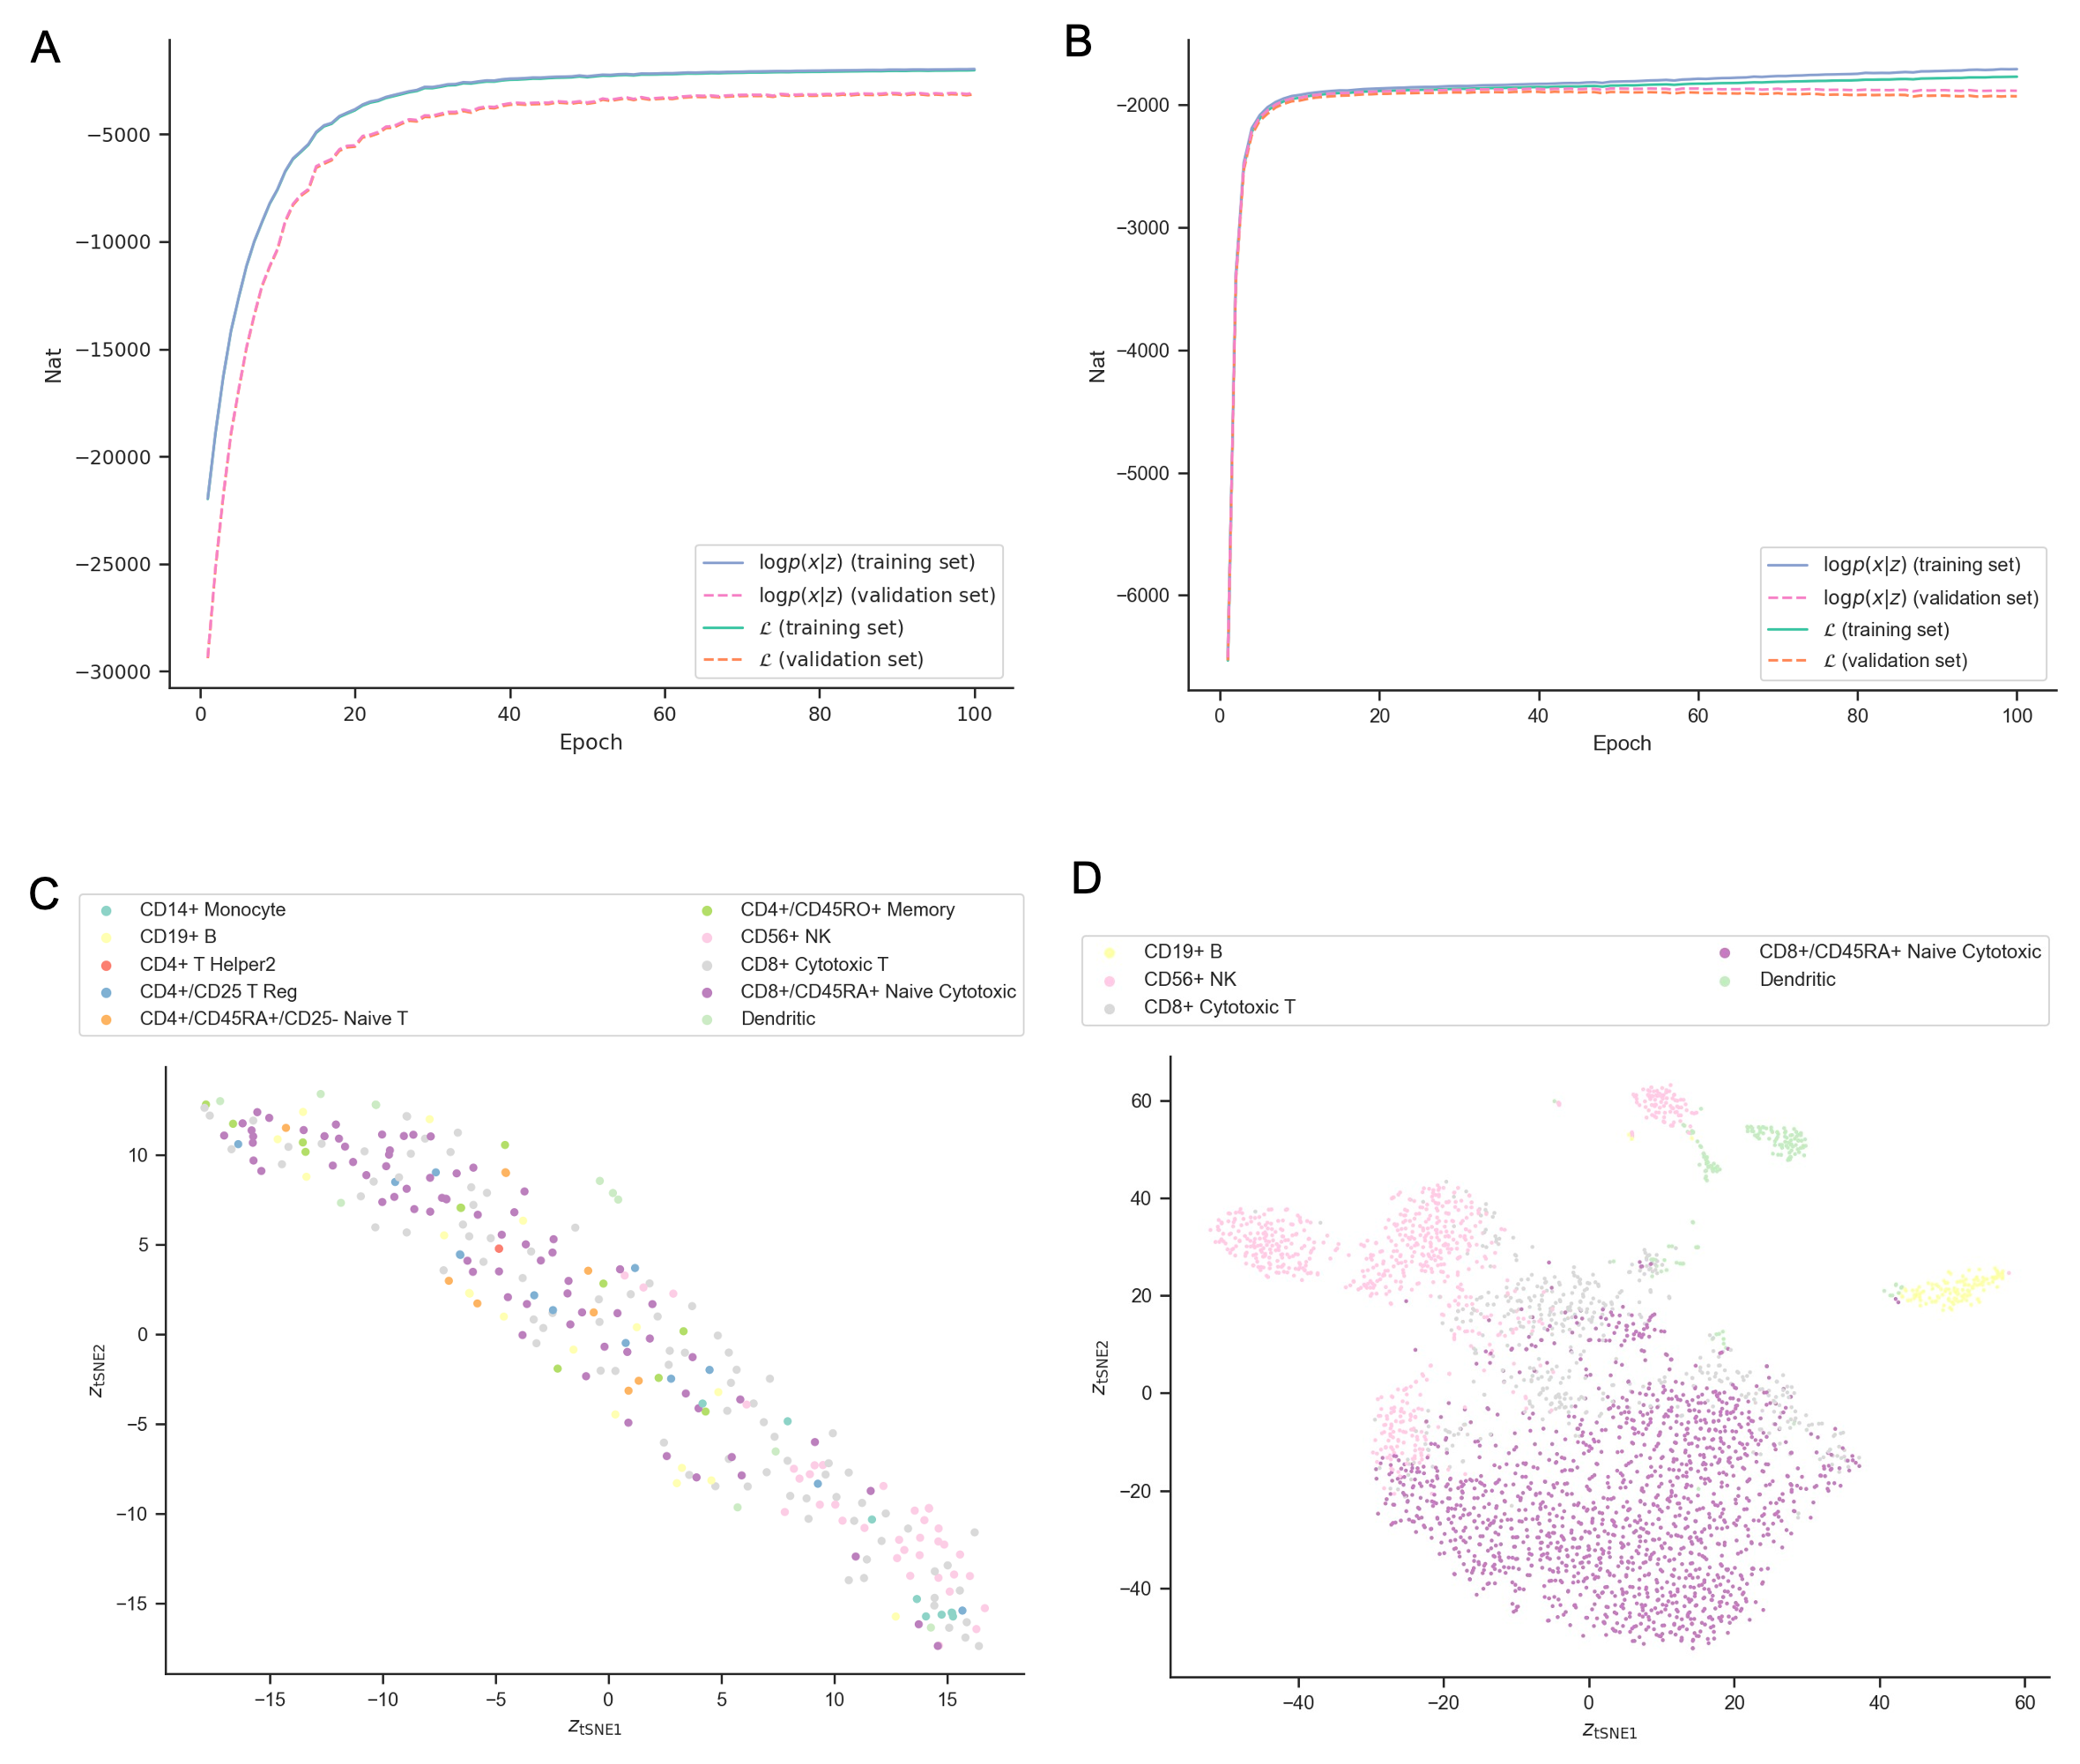
\includegraphics[width=0.70\textwidth]{02456_report/images/results_scvae.png}
    \caption{\small{\gls{scvae} model 15: learning curve (A) and \gls{tsne} visualization of the \gls{lr} (C), \gls{scvae} model 20: learning curve (B) and \gls{tsne} visualization of the \gls{lr} (D).}}
    \label{figure:cluster_training}
\end{figure*} 

\begin{table}[h]
\caption{\small{Four \gls{scvae} models test performance from 15,000 cells subset. Z = latent dimensions; H = hidden units.}}
\vspace{0.25cm}
\small
\centering
\begin{tabular}{rrrrr}
\hline
Model & Z & H & ELBO    & Rand Index \\ \hline
17     & 10                                          & 250          & -1871.9 &  0.169    \\ 
18     & 25                                          & 500          & -1890.5 & 0.188      \\ 
19     & 50                                          & 250          & -1876.4 &   0.236   \\ 
20     & 100                                          & 500         & -1880.7 &  0.212    \\ 
 \hline
\end{tabular}
\label{tab:17-20_models}
\end{table}

\noindent In figure \ref{figure:cluster_training}, the learning curve and the \gls{tsne} visualization of the \gls{lr} for models 15 and 20 are shown. 
It can be appreciated that the models trained with a larger subset of the data reach a higher value of \gls{elbo}. 
Concerning the clustering, model 20 also achieves a better Rand Index, which can be observed in the \gls{tsne} representation.\\






% ------------ ffnn --------------------
\subsection{Cell type classification using \gls{ffnn}}
\label{sec:results_ffnn}

\noindent To assess the power of \gls{scvae} to classify \gls{scrna-seq} data, a \gls{ffnn} was trained on (1) the raw count data, (2) the features resulting from applying \gls{pca} on the raw counts and (3) the \glspl{lr} generated with \gls{scvae}.
Four \gls{scvae} input sets were used, corresponding to the outperforming models in terms of \gls{elbo}, for each latent dimension tried ($Z\epsilon[10, 25, 50, 100]$). 
Likewise, for an adequate comparison, four input \gls{pca} sets were used for the \gls{ffnn} model, containing same the number of components, $k$, as latent dimensions modelled ($k\epsilon[10, 25, 50, 100]$).
All these input sets were generated using a subset of 1,300 cells of the original data set. 
A fourth type of input set was included afterwards, corresponding to the \glspl{lr} generated with \gls{scvae} using a subset of 15,000 cells (see \textit{Methods} section \ref{sec:dataset}).\\

\begin{table}[htp]
\centering
\caption{\small{Cell-type classification accuracy of test set from all \gls{ffnn} models built.
Model = \gls{scvae} model numbering used in tables
\ref{tab:16_models} and \ref{tab:17-20_models};
Subset = number of cells;
Dim = number of components (k) or latent dimensions (Z); 
H = number of hidden units used in \gls{scvae} to generate the \glspl{lr}.}}

\vspace{0.4cm}
\small
\begin{tabular}{lrrrrr} 
\hline
\multicolumn{1}{l}{Input} & \multicolumn{1}{r}{Subset} & \multicolumn{1}{r}{Model} & \multicolumn{1}{r}{Dim} & \multicolumn{1}{r}{H} & \multicolumn{1}{r}{Accuracy}  \\ 
\hline
raw  & 1,300   & -    & -    & -   & 0.655    \\
 &    &     &    &    &     \\
PCA  & 1,300    & -    & 10   & -   & 0.580    \\
     &               & -    & 25   & -   & 0.556     \\
     &               & -    & 50   & -   & 0.569    \\
     &               & -    & 100  & -   & 0.621     \\
      &    &     &    &    &     \\
scVAE  & 1,300 & 2    & 10   & 250 & 0.536      \\
       &             & 7    & 25   & 500 & 0.622     \\
       &             & 10   & 50   & 250 & 0.765      \\
       &             & 15   & 100  & 500 & 0.585    \\
        &    &     &    &    &     \\
scVAE       & 15,000  & 17 & 10   & 250 & 0.687       \\
       &               & 18 & 25   & 500 & 0.656      \\
       &               & 19 & 50   & 250 & 0.687      \\
       &               & 20 & 100  & 500 & 0.673       \\
\hline
\end{tabular}
\label{tab:ffnn_accuracies}
\end{table}

\begin{figure*}[h]
    \centering
    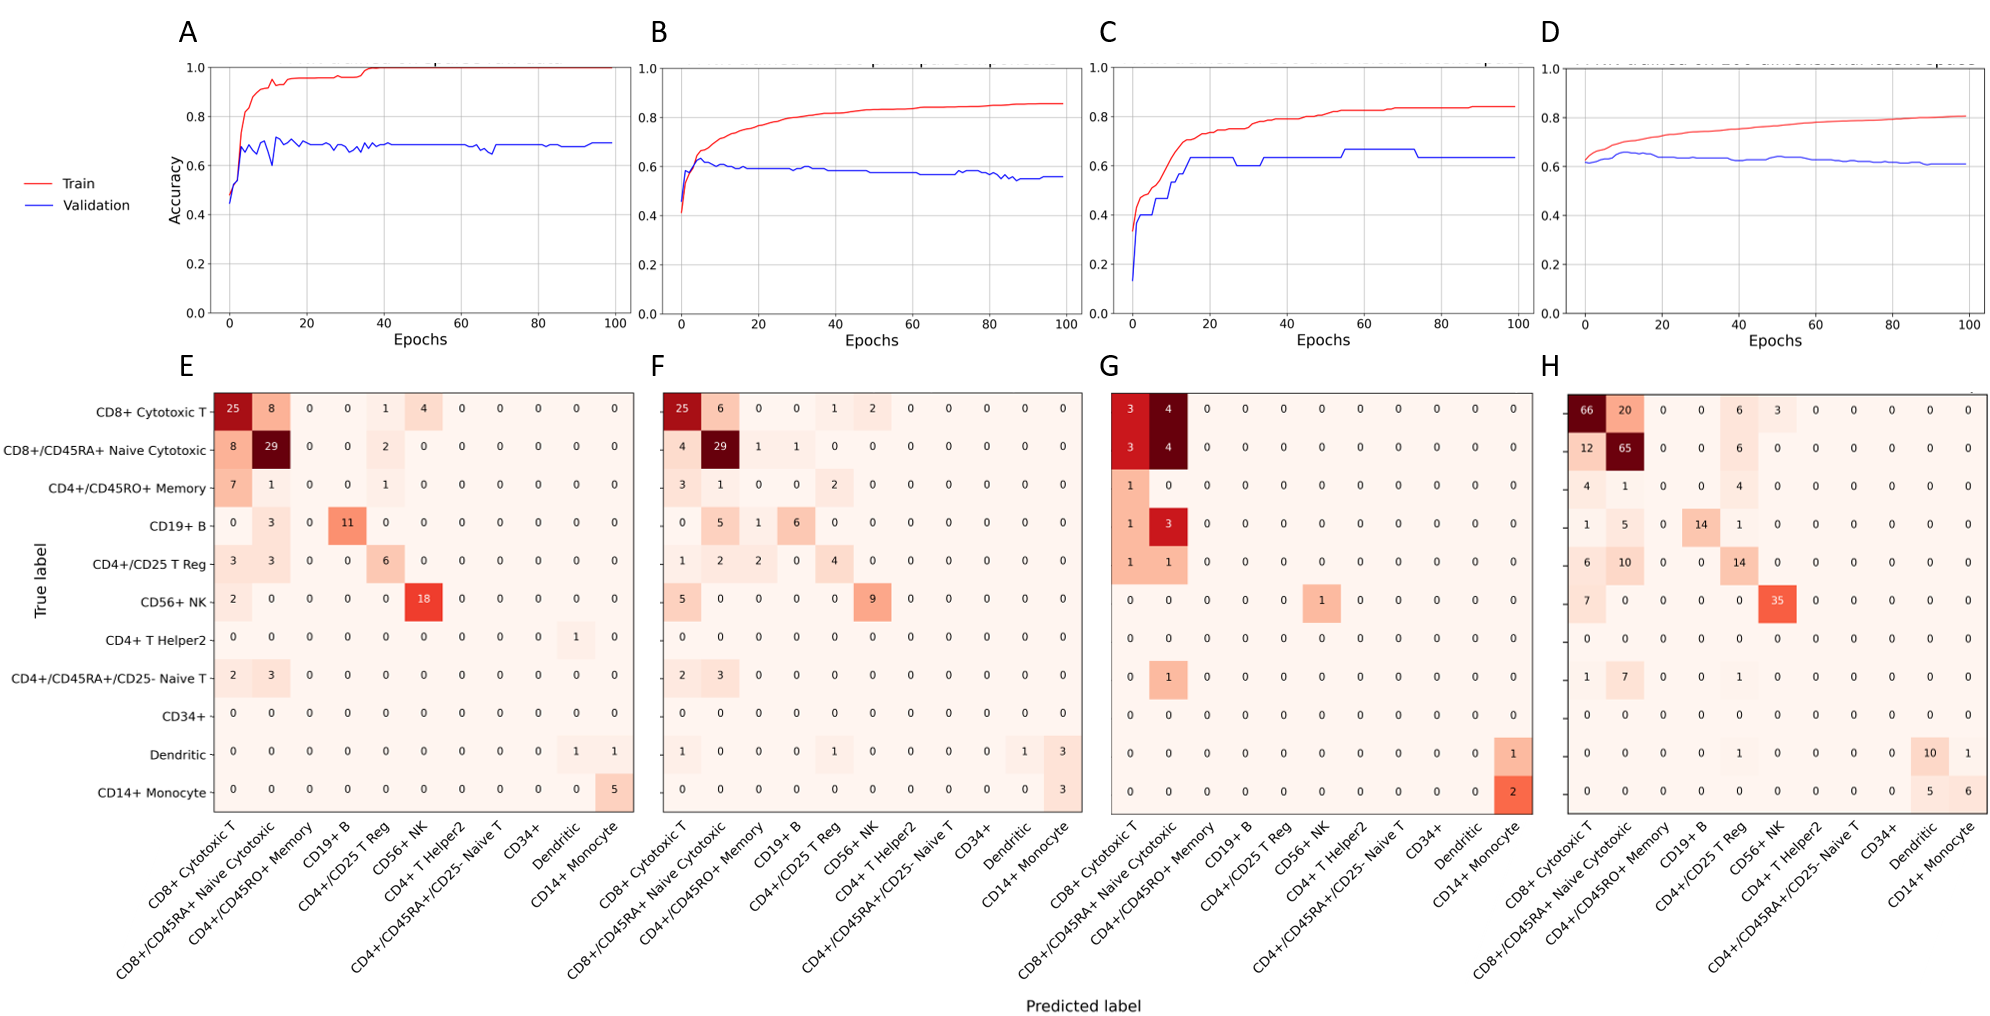
\includegraphics[width=\textwidth]{02456_report/images/results_ffnn.png}
    \caption{\small{
    \gls{ffnn} classification results.
    A-D: 
    learning curves of model trained on raw data (A), model trained on \gls{pca} features ($k=100$) (B), 
    model trained on outperforming \gls{scvae} \gls{lr} ($Z=100, H=500$) (C),
    model trained on outperforming \gls{scvae} \gls{lr} ($Z=100, H=500$) using the subset of 15000 cells (D). 
    Red curve: training accuracy; blue curve: validation accuracy. 
    E-F:
    confusion matrices of test set from the model trained on raw data (E),
    model trained on \gls{pca} features ($k=100$) (F), 
    model trained on outperforming \gls{scvae} \gls{lr} ($Z=100, H=500$) (G),
    model trained on outperforming \gls{scvae} \gls{lr} ($Z=100, H=500$) using the subset of 15,000 cells (H).
    }}
    \label{fig:ffnn_results}
    
\end{figure*}


\noindent As it can be observed in table \ref{tab:ffnn_accuracies}, the classification accuracy does not clearly differ among the input data used to train the \gls{ffnn}.
It was initially thought this outcome would be due to the small sample size used, only slight improvements were observed using as input the \gls{scvae} \glspl{lr} generated with the subset of 15,000 cells (25\% of original data set).
Moreover, the number of dimensions in the \gls{pca} or the \gls{lr} inputs does not cause any clear effect in the classification accuracy. \\

\noindent Figure \ref{fig:ffnn_results} shows the learning curves and test classification results of the \gls{ffnn} models trained \gls{scvae} outperforming model (Z=100, H=500), on \gls{pca} features with an equivalent number of components (k=100) and the raw data.
The graphs corresponding to the rest of the \gls{ffnn} models run can be found on supplementary figures S3-S6.
The \gls{ffnn} learning curves shown in figure \ref{fig:ffnn_results} reveal a considerably higher accuracy in the training process than in the validation. 
This event, slightly stronger using raw and \gls{pca}
input, is a sign of overfitting, % which is undesired and hampers the reliability of the model
that does not seem to be solved by increasing the sample size, as observed in figure \ref{fig:ffnn_results}.D. \\

\noindent Lastly, confusion matrices shown in figure \ref{fig:ffnn_results}.E-H reveal a strong class imbalance: the majority of cell types in the data set corresponds to CD8+ cytotoxic T cells. 
This event might be another reason for the low performance observed.


% ------------discussion--------------------
\section{Discussion}
\label{sec:discussion}

\noindent The \gls{scvae} model trained on 1,300 cells does not achieve pure clusters and does not reach good values of \gls{elbo}. 
For all the range of parameters tested, there is not any apparent clustering when observing the \gls{tsne} plots from the small subsets. 
The rest of the parameters used were the optimal parameters reported by Grønbech et al. 2020 \cite{gronbech2020}.
These results suggested that the selected subset of the data might need to be scaled-up, which led to the evaluation of a larger subset of 15,000 cells.\\

\noindent Modelling on the larger subset showed more differentiated clusters on the \gls{tsne} plots and the training reached \gls{elbo} values closer to zero.  
This outcome confirms that  1,300  cells  are  not  enough to obtain meaningful \glspl{lr} of the data.
Regardless of the subset size, the \gls{lr} dimension or the number of hidden units do not seem to have an effect on the quality of the computed models included in this study.
To further test the importance of the sample size, it would be interesting to see which sizes represent a good trade-off between small subsets, and thus low computational intensity, and meaningful \glspl{lr}. \\

\noindent Another aspect worth mentioning is that for all 20 models, regardless of the subset size, the learning curve reached a plateau before 50 epochs. 
This might also be an indicator that the sample size should be increased.\\

\noindent In spite of the low performance observed in \gls{scvae} models, the \glspl{lr} of the outperforming models were used to train a \gls{ffnn} to classify the cell types and compare the potential of \gls{scvae} \glspl{lr} to other inputs, such as \gls{pca} components and raw data.
Contrary to our hypothesis, the resulting classification accuracies do not show a clear difference among the three input sets used, and neither among the number of input dimensions used. \\

\noindent On one side, performing \gls{pca} prior to training the \gls{ffnn} does not improve the classification accuracy compared to direclty using raw data.
This could be due to the fact that the first 100 principal components can only explain approximately 20\% of the variance, as shown in supplementary figure S2.
This suggests the use of \gls{pca} might not be helpful in this case.
On the other side, using the \gls{lr} obtained from \gls{scvae} does not seem to improve the accuracy either, regardless of the subset size, by direct comparison to the \gls{pca} components. 
Moreover, a strong sign of overfitting has been observed in all \gls{ffnn} models. \\ 

\noindent The subset size might be one of the main causes for this outcome, as the model trained on the \gls{lr} generated with the larger subset shows a slight improvement in accuracy and overfitting compared to the model trained on the \gls{lr} generated with the smaller subset. 
Unfortunately, due to unavailability of a raw subset of 15,000 cells, as described in \textit{Methods} section \ref{sec:dataset}, direct comparisons between the performance of a \gls{ffnn} classifier using raw data, \gls{pca} components or \gls{scvae} \glspl{lr} on the larger subset cannot be precisely done.
Nevertheless, and in line with the insights revealed by \gls{scvae} models, these results still suggest that training the \gls{ffnn} on a larger subset will lead to better performances. \\

\noindent The classification outcome could have also been affected by a strong class imbalance, probably resulting from sampling a small fraction of the original data set (2\%).
An assessment of class imbalance was thereby conducted and, as it can be observed in supplementary figure S7,  an inherent class imbalance was observed in the complete data set.
This is thus reflected in the subset, but it is not an effect resulting from sub-sampling.
Still, this imbalance might be hampering the classification results. \\ 

\noindent Overall, we can not conclude in this study that the use of \gls{scvae} \glspl{lr} improves the performance of cell-type classification.
However, the findings obtained shed light onto the fact that increasing the sample size can lead to higher \gls{ffnn} classification accuracies. 
Larger subsets, as mentioned in \textit{Methods} section \ref{sec:dataset}, could not be used in this study due to limited computational resources.
Therefore, further studies following the same methodology but on larger data sets could be interesting and beneficial to appropriately assess the true potential of \glspl{vae}, and particularly \gls{scvae}, to classify high-dimensional, sparse data such as \gls{scrna-seq} data.
\\



% ----- acknowledgments and author participation ------
\section{Acknowledgments}

\noindent The authors of the project would like to acknowledge the help and guidance on \gls{scvae} received from C. H. Grønbech, as well as the supervision from O. Winther.

\section{Author contributions}

\noindent All the authors of the project contributed equally to all parts of the project: (1) study design, (2) model creation and coding, (3) results interpretation and (4) poster design and article writing. \\

\noindent Begoña Bolós Sierra -  s193036\\
Felix Pacheco Pastor - s192496\\
Paula Rodríguez García - s192448\\
Laura Sans Comerma - s192437

% -------- supp materials -------
\section{Supplementary materials}
All the analyses and results conducted and generated in this project can be found online at \href{https://github.com/laurasansc/02456_scVAE}{02456\_scVAE repository}.
Supplementary figures can be found on the supplementary PDF document attached to this report.
A poster containing the main insights about this work can be found in \href{https://github.com/laurasansc/02456_scVAE/blob/main/docs/poster/scVAE_poster.pdf}{Github}.
\newpage
% -------------refs-------------------
\bibliographystyle{IEEEbib}
\bibliography{refs}




\end{document}